\documentclass[11pt,a4paper]{book}
\usepackage{Appunti_universitari}

\begin{document}
\title{Programmazione C++ \\
	\large Riassunto di "The C++ Programming Language" \\
	4a edizione \\ 
	\textit{Bjarne Stroustrup}}
\author{Jacopo De Angelis}
\maketitle

\pagebreak
\tableofcontents
\pagebreak

\begin{LARGE}
Programma esteso
\end{LARGE}

\begin{itemize}
	\item Introduzione al C++.
	\item Concetti base di programmazione C++
	\begin{itemize}
		\item tipi di dati, puntatori,  reference, scoping
		\item casting,
	\end{itemize}

	\item C++ come linguaggio ad oggetti
	\begin{itemize}
		\item classi, costruttori e distruttori, overloading, metodi friend
		\item inline, constness"           
	\end{itemize}	
	\item Concetti avanzati di programmazione C++
	\begin{itemize}
		\item overloading degli operatori
		\item metodi virtual, abstract, polimorfismo
		\item ereditarietà
	\end{itemize}
	\item Programmazione generica
	\begin{itemize}
		\item template
		\item iteratori
	\end{itemize}	
	\item La libreria Standard (STL)
	\begin{itemize}
		\item Le classi container
		\item Gli algoritmi
		\item Funtori
		\item Multithread
	\end{itemize}	
	\item Uso delle librerie esterne
	\begin{itemize}
		\item Librerie statiche
		\item Librerie dinamiche
		\item La libreria OpenMP
	\end{itemize}	
	\item I nuovi standard C++11, C++14
	
	\item Applicazioni GUI
	\begin{itemize}
		\item Ambiente di sviluppo QT Creator
		\item Sviluppo di interfacce grafiche
		\item Gestione degli eventi
		\item Le librerie Qt, QTWidget...
	\end{itemize}
\end{itemize}
\pagebreak

\chapter{Principi base}
\section{Le basi}
C++ è un linguaggio compilato. Il processo di compilazione è unione dei file è il seguente:
\begin{figure}[h!]
	\begin{center}
		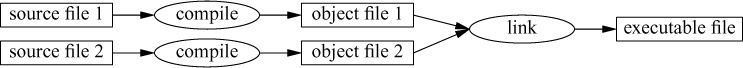
\includegraphics[scale=0.6]{img/001.jpg}
		\caption{Processo di compilazione e unione}
		\label{fig: 001}
	\end{center}
\end{figure}
Il programma è creato per uno specifico sistema operativo. \textbf{C++ è source portable}. Lo standard ISO C++ specifica due entità:
\begin{itemize}
	\item \textbf{Caratteristiche del linguaggio core}: tipi built-in e loop
	\item \textbf{Librerie standard}: container e operazioni I/O
\end{itemize}
\textbf{C++ è un linguaggio fortemente tipizzato e statico}.

\subsection{Hello, World!}
\lstinputlisting[language=C++]{code/001.cpp}\label{code: 001}
Cose che possiamo notare:
\begin{itemize}
	\item \#include <iostream>: include la libreria iostream, ovvero la libreria di I/O
	\item <<: prescrive in inserire il secondo argomento nel primo
	\item //: Commento su singola linea
	\item std::cout: standard output, fa parte del namespace della libreria standard
\end{itemize}

\lstinputlisting[language=C++]{code/002.cpp}\label{code: 002}
Void indica che la funzione non ha valori di ritorno.

\subsection{Tipi, variabili e aritmetica}
Una dichiarazione è una stringa di codice che introduce il nome del programma. É costituita da tipo e nome. I tipi primitivi di C++ sono:
\begin{itemize}
	\item bool: 
	\item char
	\item int
	\item double
\end{itemize}
In più int, char e double possono anche avere dei modificatori:
\begin{itemize}
	\item long
	\item short
	\item signed
	\item unsigned
\end{itemize}

Le combinazioni sono:
\begin{table}[]
\resizebox{\textwidth}{!}{%
\begin{tabular}{|c|c|c|}
\hline
{\color[HTML]{333333} \textbf{Data type}} & {\color[HTML]{333333} \textbf{Size (bit)}} & {\color[HTML]{333333} \textbf{Range}}                 \\ \hline
short int                                 & 16                                         & -32,768 to 32,767                                     \\ \hline
unsigned short int                        & 16                                         & 0 to 65,535                                           \\ \hline
unsigned int                              & 32                                         & 0 to 4,294,967,295                                    \\ \hline
int                                       & 32                                         & -2,147,483,648 to 2,147,483,647                       \\ \hline
long int                                  & 32                                         & -2,147,483,648 to 2,147,483,647                       \\ \hline
unsigned long int                         & 32                                         & 0 to 4,294,967,295                                    \\ \hline
long long int                             & 64                                         & -(2\textasciicircum{}63) to (2\textasciicircum{}63)-1 \\ \hline
unsigned long long int                    & 64                                         & 0 to 18,446,744,073,709,551,615                       \\ \hline
signed char                               & 8                                          & -128 to 127                                           \\ \hline
unsigned char                             & 8                                          & 0 to 255                                              \\ \hline
float                                     & 32                                         &                                                       \\ \hline
double                                    & 64                                         &                                                       \\ \hline
long double                               & 96                                         &                                                       \\ \hline
wchar\_t                                  & 16 o 32                                    & 1 wide character                                      \\ \hline
\end{tabular}%
}
\end{table}
\emph{sizeof(var)} permette di ottenere la dimensione della variabile.

Aritmetica:
\begin{itemize}
	\item x+y
	\item +x: +1
	\item x–y
	\item –x: -1
	\item x*y
	\item x/y
	\item x\%y: modulo della divisione
	\item
	\item x+=y: x = x+y
	\item ++x: x = x+1
	\item x–=y: x = x-y
	\item ––x: x = x-1
	\item x*=y: x = x*y
	\item x/=y: x = x/y
	\item x\%=y: x = x\%y
\end{itemize}

Comparazione:
\begin{itemize}
	\item x==y: equal
	\item x!=y: not equal
	\item x<y: less than
	\item x>y: greater than
	\item x<=y: less than or equal
	\item x>=y: greater than or equal
\end{itemize}

C++ esegue automaticamente la conversione tra tipi nelle operazioni aritmetiche.

\textbf{Code quality}: mai inizializzare a vuoto se possibile. I tipi definiti dall'utente possono avere un'inizializzazione implicita. \label{Code quality: 001}

\subsection{Costanti}
C++ supporta due tipi di costanti:
\begin{itemize}
	\item const: la varibaile è una costante, non viene modificata. Viene usata generalmente per specificare le interfacce, in questo modo i dati possono essere passati alle funzioni senza che queste possano modificarli
	\item constexpr: la variabile verrà valutata durante la compilazione. Usata soprattutto per specificare le costanti, per permettere il posizionamento dei dati in memoria dove è difficile che vengano corrotti, e per performance
\end{itemize}
\lstinputlisting[language=C++]{code/003.cpp}\label{code: 003}
Affinchè una costante venga valutata dal compilatore, essa deve essere definita come constexpr. Per essere una constexpr, la funzione deve essere molto semplice: deve avere solo il return. Le constexpr possono essere chiamate anche a runtime, in questo caso si comportano normalmente.

Le constexpr sono obbligatorie in certi casi che vedremo poi. In altri casi sono usate per performance. Nel caso un oggetto sia immutabile è necessario pensarci.

\subsection{Puntatori, array e loop}
\subsubsection{Puntatori}
Un array viene dichiarato come \emph{char v[6];} mentre un puntatore \emph{char* p}. Gli array partono da 0. L'arra deve avere una lunghezza costante. Un puntatore può contenere l'indirizzo di un oggetto del tipo appropriato.
\lstinputlisting[language=C++]{code/004.cpp}\label{code: 004}

Possiamo vedere che * indica "contenuto di" mentre \& indica "indirizzo di".
\begin{figure}[h!]
	\begin{center}
		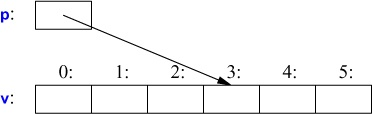
\includegraphics[scale=0.6]{img/002.jpg}
		\caption{Puntatori e indirizzi}
		\label{fig: 002}
	\end{center}
\end{figure}

\subsubsection{Loop}
Ecco due implementazioni del ciclo for:
\lstinputlisting[language=C++]{code/005.cpp}\label{code: 005}
\lstinputlisting[language=C++]{code/006.cpp}\label{code: 006}

Una delle prime cose che notiamo è \emph{auto}: questa parola chiave si occupa di fare inferenza riguardo il contenuto della variabile, serve per non dichiarare esplicitamente che variabile primitiva. Può anche essere utilizzata come tipo di ritorno delle funzioni. Ottima per collegare ad una sola funzione o variabile temporanea più variabili con una notazione generica.

In questi due esempi copiamo il primo vettore nel secondo, ma se volessimo solo dire "incrementa ciò che c'è dentro al vettore ma senza creare una nuova variabile per farlo"? Dovremmo usare un ciclo che implementa dei puntatori e degli indirizzi:
\lstinputlisting[language=C++]{code/007.cpp}\label{code: 007}

In una dichiarazione il suffisso \& significa "reference a". Una "reference" è simile ad un puntatore, eccetto che non ti serve il prefisso * per accedere al valore puntato. In più una reference deve puntare sempre allo stesso oggetto dopo la sua inizializzazione.

Quando usati nelle di dichiarazioni, gli operatori \&, * e [] sono chiamati "operatori di dichiarazione":
\lstinputlisting[language=C++]{code/008.cpp}\label{code: 008}

Un altro tipo di loop è il while:
\lstinputlisting[language=C++]{code/009.cpp}\label{code: 009}

\subsection{Test di verità}
I test di verità, oltre agli operatori ==, != ecc. abbiamo delle funzioni che si occupano di modificare il flusso del programma in base ai valori. Sono if, while e switch:
\lstinputlisting[language=C++]{code/010.cpp}\label{code: 010}
\lstinputlisting[language=C++]{code/011.cpp}\label{code: 011}

\subsection{Tipi definiti dall'utente}
\subsubsection{Strutture}
Il primo modo per costruire un nuovo tipo è, spesso, il riorganizzare i dati in una struttura.
\lstinputlisting[language=C++]{code/012.cpp}\label{code: 012}
Qua possiamo vedere l'implementazione di un vettore tramite struct e la sua inizializzazione.

Per inizializzarlo dobbiamo però creare un'apposita funzione:
\lstinputlisting[language=C++]{code/013.cpp}\label{code: 013}
In questo modo la funzione vector\_init ottiene un puntatore alla variabile creata esternamente e il numero di elementi. Il fatto di usare Vector\& serve in modo da ottenere una variabile non locale ma con effetti sulla variabile originale.

L'operatore new alloca memoria per la variabile. Un tipico uso di Vector è questo:
\lstinputlisting[language=C++]{code/014.cpp}\label{code: 014}

Notiamo che questo vettore non è, ovviamente, il vector della libreria standard.

\subsubsection{Classi}
Qua veniamo a conoscenza della differenza tra interfaccia e implementazione di una classe. L'interfaccia è accessibile a tutti, l'implementazione è inaccessibile se non tramite appositi metodi.

La classe è definita da una serie di membri (funzioni, dati o strutture). Questi sono privati, accessibili solo tramite la loro interfaccia pubblica.
\lstinputlisting[language=C++]{code/015.cpp}\label{code: 015}

Una funzione con lo stesso nome della classe è chiamata "costruttore" e ha la funzione di creare la classe con i parametri passati.

\subsubsection{Enumerazioni}
\lstinputlisting[language=C++]{code/016.cpp}\label{code: 016}
Le enumerazioni sono usate per rappresentare un riotto set di valori. Sono usate per rendere il codice più leggibile e meno prono ad errori. Notare che queste enumerazioni sono fortemente tipizzate, ad esempio:
\lstinputlisting[language=C++]{code/017.cpp}\label{code: 017}

Se l'enumerazione non è basata su di una classe ma su di un tipo primitivo basta rimuovere "class".

\subsection{Modularità}
\subsubsection{Compilazione separata}
C++ supporta la compilazione separata dei vari file. Può essere usato per dividere il programma in blocchi di codice semi indipendenti. Questa separazione può essere usata per ridurre il tempo di compilazione richiesto.

Spesso inseriamo le dichiarazioni che specificano l'interfaccia di un modulo in un file denominato header (*.h). Ad esempio possiamo vedere qua prima l'header Vector.h e poi la sua implementazione:
\lstinputlisting[language=C++]{code/018.cpp}\label{code: 018}
Per far sì che il compilatore assicuri la consistenza del codice, anche nella deifnizione viene incluso l'header.

Qua il suo uso:
\lstinputlisting[language=C++]{code/019.cpp}\label{code: 019}

I file possono essere compilati in maniera indipendente, lo schema è più o meno questo:
\begin{figure}[h!]
	\begin{center}
		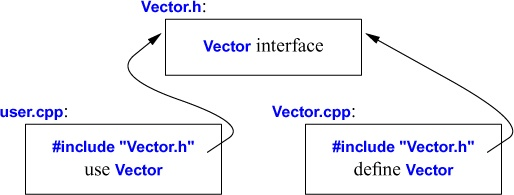
\includegraphics[scale=0.6]{img/003.jpg}
		\caption{Uso dell'header}
		\label{fig: 003}
	\end{center}
\end{figure}

\subsubsection{Namespace}
C++ offre anche i namespace come meccanismo per esprimere alcune dichiarazioni che appartengono allo stesso gruppo senza che vadano in conflitto con altri. Per esempio, potremmo sperimentare con il nostro numero complesso e includerlo nel main in modo che non vada in conflitto con la versione originale:
\lstinputlisting[language=C++]{code/020.cpp}\label{code: 020}

Un modo per accedere alle variabili di altri namespace è \emph{nome\_del\_namespace::funzione/variabile}.Per avere accesso a tutti i nomi della libreria standard possiamo usare la direttiva using, ad esempio \emph{using namespace std;}

\subsection{Gestione degli errori}
\subsubsection{Eccezioni}
Lo schema è il classico try-throw-catch:
\begin{itemize}
	\item Il codice che potrebbe generare un'eccezione viene messo all'interno di un blocco try
	\item L'eccezione viene lanciata con throw
	\item L'eccezione viene gestita da un catch
\end{itemize}

\lstinputlisting[language=C++]{code/021.cpp}\label{code: 021}

\subsubsection{Invarianti}
Prendiamo un esempio classico: cercare di inizializzare un array con un numero negativo. Questa situazione può essere segnalata con un'eccezione della libreria standard, length\_error. In più se il compilatore non riesce ad allocare memoria darà come risposta un'eccezione bad\_alloc. Quindi, il codice diventa:
\lstinputlisting[language=C++]{code/022.cpp}\label{code: 022}

\subsubsection{Asserzioni statiche}
Le eccezioni riportano errori a runtime. Se un errore può essere trovato a tempo di compilazione allora è meglio individuarlo in quel momento. Per farlo possiamo usare le asserzioni statiche. L'importante è che vengano usate con un'espressione costante. Ad esempio:
\lstinputlisting[language=C++]{code/023.cpp}\label{code: 023}

\chapter{Astrazione}
\section{Classi}
Ci sono tre tipi di classi:
\begin{enumerate}
	\item classi concrete
	\item classi astratte
	\item classi nella gerarchia
\end{enumerate}
\subsubsection{Classi concrete}
L'idea è che si comporti esattamente come un tipo built-in. La caratteristiche che definisce un tipo concreto è che la rappresentazione fa parte della definizione. 

\paragraph{Un tipo aritmetico}
Questo è un tipo tipo aritmetico definito dall'utente:
\lstinputlisting[language=C++]{code/024.cpp}\label{code: 024}

Un costruttore che può essere invocato senza argomenti è chiamato "costruttore di default". Definendo un costruttore di default si stabilisce che non possono esistere variabili non inizializzate.
const sulla funzione definisce che queste funzioni non modificano l'oggetto con il quale sono chiamate.

Molte operazioni non richiedono accesso diretto alla rappresentazione, quindi possono essere definite separatamente dalla definizione della classe.

\paragraph{Container}
Un container è un oggetto che contiene una collezione di elementi, ad esempio un vettore. Pro di Vector: offre controllo di accesso sugli indici e offre una comoda funzione size. Difetto: alloca gli elementi usando new ma non li dealloca mai. C++ offre un'interfaccia per il garbage collector ma non viene usata automaticamente, quindi in certi casi potremmo trovarci a preferire un approccio più preciso. Questo meccanismo è un \emph{destructor}:
\lstinputlisting[language=C++]{code/025.cpp}\label{code: 025}

Il nome del destructor è l'operazione complementare ~ seguita dal nome della classe. É il complemento del costruttore. Il costruttore alloca la memoria nell'heap usando l'operatore new. Il distruttore pulisce usando l'operatore delete.

La tecnica di acquisire le risorse in un costruttore e rilasciarle in un distruttore è nota come \textbf{"Resource Acquisition Is Initialization" o RAII}. Ciò permette di nascondere le operazioni new e delete, separando l'implementazione dall'astrazione.

\paragraph{Inizializzare i container}
Un container esiste per contenere elementi, dobbiamo quindi avere dei metodi comodi per inserirveli. Possiamo creare un vettore con il numero appropriato di elementi e poi aggiungendoli, ma solitamente ci sono modi più eleganti.
Due modi possono essere:
\begin{itemize}
	\item initalize
	\item push\_back(): aggiunge un elemento in fondo alla lista
\end{itemize}

\lstinputlisting[language=C++]{code/026.cpp}\label{code: 026}

Il ciclo for è stato scelto per avere d solo nel suo scope e non occupare memoria dopo. La fine dello stream è decretata da un end-of-file (EOF) o da un errore di formattazione.

\subsubsection{Tipi astratti}


\end{document}